%%%%%%%%%%%%%%%%%%%%%%%%%%%%%%%%%%%%%%%%%
% Beamer Presentation
% LaTeX Template
% Version 2.0 (March 8, 2022)
%
% This template originates from:
% https://www.LaTeXTemplates.com
%
% Author:
% Vel (vel@latextemplates.com)
%
% License:
% CC BY-NC-SA 4.0 (https://creativecommons.org/licenses/by-nc-sa/4.0/)
%
%%%%%%%%%%%%%%%%%%%%%%%%%%%%%%%%%%%%%%%%%

%----------------------------------------------------------------------------------------
%	PACKAGES AND OTHER DOCUMENT CONFIGURATIONS
%----------------------------------------------------------------------------------------

\documentclass[compress]{beamer}
%\usepackage{beamerthemesplit}
\usepackage{hyperref}
\usepackage{color}                  %para gr\'{a}ficos, colores ....
\usepackage{amssymb}                %para simbolos Ams
\usepackage{amsmath}                %para letras barradas
\usepackage{enumerate}              %para definir los estilos en las enumeraciones
\usepackage[english,spanish,activeacute]{babel} %imprime palabras por defecto en castellano
\uselanguage{Spanish}
\languagepath{Spanish}
\usepackage{amsfonts,amsbsy}

\usepackage{epsfig}
\usepackage{graphics}               %para introducir archivos eps
\usepackage{graphicx}               %para gr\'{a}fcos
\usepackage[utf8]{inputenc}

%\graphicspath{{Images/}{./}} % Specifies where to look for included images (trailing slash required)

\usepackage{booktabs} % Allows the use of \toprule, \midrule and \bottomrule for better rules in tables


\usepackage[dvipsnames, table, xcdraw]{xcolor}

\usepackage[numbers, sort&compress]{natbib}
\setlength{\bibsep}{10pt}
%\usepackage[natbibapa]{apacite}
%\usepackage{natbib}                % para usar el teclado normalmente
\usepackage{svg}
\usepackage{subcaption}
\usepackage{float}
\usepackage{caption}
\usepackage{listings}
\usepackage{listingsutf8}

\usepackage[T1]{fontenc}
\usepackage[utf8]{inputenc}
\usepackage{array}
\definecolor{ventaja}{RGB}{235, 255, 235} 
\definecolor{desventaja}{RGB}{255, 245, 235} 

\usepackage{minted}
\usemintedstyle{colorful}

% Si alguno de estos paquetes no los vas a usar, mejor los quitas:
\usepackage{amssymb}               % para cargar las fuentes de la A.M.S.
\usepackage{amsmath}               % para usar letras griegas en negrita
\usepackage{amsthm}                % mejora los entornos tipo-teorema y proof
\usepackage{mathptmx}              % fuente Times
%\usepackage{lmodern}              % fuente Times
\usepackage{tikz}                  % para los dibujos
\usetikzlibrary{babel}  
\usepackage[absolute,overlay]{textpos}  

% 2. Ahora sí podemos vincular la proposición a ese contador
\newtheorem{proposition}[theorem]{Proposición}

%------ Conjuntos de números
\newcommand\N{\mathbb{N}}
\newcommand\Z{\mathbb{Z}}
\newcommand\R{\mathbb{R}}
\newcommand\C{\mathbb{C}}
%----------------------------------------------------------------------------------------
%	SELECT LAYOUT THEME
%----------------------------------------------------------------------------------------

% Beamer comes with a number of default layout themes which change the colors and layouts of slides. Below is a list of all themes available, uncomment each in turn to see what they look like.

%\usetheme{default}
%\usetheme{AnnArbor}
%\usetheme{Antibes}
%\usetheme{Bergen}
%\usetheme{Berkeley}
%\usetheme{Berlin}
%\usetheme{Boadilla}
%\usetheme{CambridgeUS}
%\usetheme{Copenhagen}
%\usetheme{Darmstadt}
%\usetheme{Dresden}
\usetheme{Frankfurt}
%\usetheme{Goettingen}
%\usetheme{Hannover}
%\usetheme{Ilmenau}
%\usetheme{JuanLesPins}
%\usetheme{Luebeck}
%\usetheme{Madrid}
%\usetheme{Malmoe}
%\usetheme{Marburg}
%\usetheme{Montpellier}
%\usetheme{PaloAlto}
%\usetheme{Pittsburgh}
%\usetheme{Rochester}
%\usetheme{Singapore}
%\usetheme{Szeged}
%\usetheme{Warsaw}

%----------------------------------------------------------------------------------------
%	SELECT COLOR THEME
%----------------------------------------------------------------------------------------

% Beamer comes with a number of color themes that can be applied to any layout theme to change its colors. Uncomment each of these in turn to see how they change the colors of your selected layout theme.

%\usecolortheme{albatross}
%\usecolortheme{beaver}
%\usecolortheme{beetle}
%\usecolortheme{crane}
%\usecolortheme{dolphin}
%\usecolortheme{dove}
%\usecolortheme{fly}
%\usecolortheme{lily}
%\usecolortheme{monarca}
%\usecolortheme{seagull}
%\usecolortheme{seahorse}
%\usecolortheme{spruce}
%\usecolortheme{whale}
%\usecolortheme{wolverine}

%----------------------------------------------------------------------------------------
%	SELECT FONT THEME & FONTS
%----------------------------------------------------------------------------------------

% Beamer comes with several font themes to easily change the fonts used in various parts of the presentation. Review the comments beside each one to decide if you would like to use it. Note that additional options can be specified for several of these font themes, consult the beamer documentation for more information.

\usefonttheme{default} % Typeset using the default sans serif font
%\usefonttheme{serif} % Typeset using the default serif font (make sure a sans font isn't being set as the default font if you use this option!)
%\usefonttheme{structurebold} % Typeset important structure text (titles, headlines, footlines, sidebar, etc) in bold
%\usefonttheme{structureitalicserif} % Typeset important structure text (titles, headlines, footlines, sidebar, etc) in italic serif
%\usefonttheme{structuresmallcapsserif} % Typeset important structure text (titles, headlines, footlines, sidebar, etc) in small caps serif

%------------------------------------------------

%\usepackage{mathptmx} % Use the Times font for serif text
\usepackage{palatino} % Use the Palatino font for serif text

%\usepackage{helvet} % Use the Helvetica font for sans serif text
\usepackage[default]{opensans} % Use the Open Sans font for sans serif text
%\usepackage[default]{FiraSans} % Use the Fira Sans font for sans serif text
%\usepackage[default]{lato} % Use the Lato font for sans serif text

%----------------------------------------------------------------------------------------
%	SELECT INNER THEME
%----------------------------------------------------------------------------------------

% Inner themes change the styling of internal slide elements, for example: bullet points, blocks, bibliography entries, title pages, theorems, etc. Uncomment each theme in turn to see what changes it makes to your presentation.

%\useinnertheme{default}
\useinnertheme{circles}
%\useinnertheme{rectangles}
%\useinnertheme{rounded}
%\useinnertheme{inmargin}

%----------------------------------------------------------------------------------------
%	SELECT OUTER THEME
%----------------------------------------------------------------------------------------

% Outer themes change the overall layout of slides, such as: header and footer lines, sidebars and slide titles. Uncomment each theme in turn to see what changes it makes to your presentation.

%\useoutertheme{default}
%\useoutertheme{infolines}
%\useoutertheme{miniframes}
%\useoutertheme{smoothbars}
%\useoutertheme{sidebar}
%\useoutertheme{split}
%\useoutertheme{shadow}
%\useoutertheme{tree}
%\useoutertheme{smoothtree}

%\setbeamertemplate{footline} % Uncomment this line to remove the footer line in all slides
%\setbeamertemplate{footline}[page number] % Uncomment this line to replace the footer line in all slides with a simple slide count

%\setbeamertemplate{navigation symbols}{} % Uncomment this line to remove the navigation symbols from the bottom of all slides

%----------------------------------------------------------------------------------------
%	PRESENTATION INFORMATION
%----------------------------------------------------------------------------------------

\title[Short Title]{Análisis Isogeométrico} % The short title in the optional parameter appears at the bottom of every slide, the full title in the main parameter is only on the title page

%\subtitle{Optional Subtitle} % Presentation subtitle, remove this command if a subtitle isn't required

\author[Carlos Palomera Oliva]{Carlos Palomera Oliva} % Presenter name(s), the optional parameter can contain a shortened version to appear on the bottom of every slide, while the main parameter will appear on the title slide


\institute{ {\centering 
\includegraphics[scale=0.35]{ciencias.png}}\\ 
{\centering 
\includegraphics[scale=0.45]{logoUZ.png}}
\\[1em] % Añade un salto de línea con un poco de espacio tras el logo
{\small \textbf{Tutores:} Álvaro Pé de la Riva y \\ Carmen Rodrigo Cardiel}
}


\date[\today]{\today} % Presentation date or conference/meeting name, the optional parameter can contain a shortened version to appear on the bottom of every slide, while the required parameter value is output to the title slide

%----------------------------------------------------------------------------------------

\begin{document}

%----------------------------------------------------------------------------------------
%	TITLE SLIDE
%----------------------------------------------------------------------------------------

\begin{frame}
	\titlepage % Output the title slide, automatically created using the text entered in the PRESENTATION INFORMATION block above
\end{frame}

%----------------------------------------------------------------------------------------
%	TABLE OF CONTENTS SLIDE
%----------------------------------------------------------------------------------------

% The table of contents outputs the sections and subsections that appear in your presentation, specified with the standard \section and \subsection commands. You may either display all sections and subsections on one slide with \tableofcontents, or display each section at a time on subsequent slides with \tableofcontents[pausesections]. The latter is useful if you want to step through each section and mention what you will discuss.

\begin{frame}
	\frametitle{Índice} % Slide title, remove this command for no title
	\scriptsize
	\tableofcontents % Output the table of contents (all sections on one slide)
	%\tableofcontents[pausesections] % Output the table of contents (break sections up across separate slides)
\end{frame}

%----------------------------------------------------------------------------------------
%	PRESENTATION BODY SLIDES
%----------------------------------------------------------------------------------------

\section{Introducción} % Sections are added in order to organize your presentation into discrete blocks, all sections and subsections are automatically output to the table of contents as an overview of the talk but NOT output in the presentation as separate slides

%------------------------------------------------

\subsection{Contexto y relación con el método de elementos finitos}

\begin{frame}
    \frametitle{Comparación}

    % --- BLOQUE DE LA IMAGEN (TEXTBLOCK) ---
    \begin{textblock*}{10.8cm}(1cm, 5.7cm) 
        \only<2-3>{
            \begin{figure}
                \captionsetup[subfigure]{skip=0pt, font=scriptsize} 
                \centering
                \begin{subfigure}{0.32\textwidth}
                    \centering
					{\tiny
                    \includesvg[width=\linewidth]{bases_fem_p1.svg}
					}

					\vspace{-10pt}
					\caption{Base FEM, p=1.}
                \end{subfigure}
                \hfill
                \begin{subfigure}{0.32\textwidth}
                    \centering
					{\tiny
                    \includesvg[width=\linewidth]{bases_fem_p2.svg}
					}

					\vspace{-10pt}
					\caption{Base FEM, p=2.}
                \end{subfigure}
                \hfill
                \begin{subfigure}{0.32\textwidth}
                    \centering
					{\tiny
                    \includesvg[width=\linewidth]{funciones_base_NURBS_2.svg}
					}

					\vspace{-10pt}
					\caption{Base NURBS, p=2.}
                \end{subfigure}
            \end{figure}
        }
    \end{textblock*}

    % --- TABLA CORREGIDA ---
    \begin{table}[htbp]
        \centering
        \renewcommand{\arraystretch}{1.3}
        \scriptsize 
        
        % p{...} alinea por la parte superior por defecto. 
        % Al usar \raggedright evitamos saltos de línea raros.
        \begin{tabular}{>{\raggedright\arraybackslash}p{2.4cm} >{\raggedright\arraybackslash}p{4cm} >{\raggedright\arraybackslash}p{4cm}}
            \toprule
            \textbf{Criterio} & \textbf{FEM Clásico} & \textbf{IGA} \\ 
            \midrule
            
            \textbf{Geometría} & 
            \cellcolor{desventaja} \textbf{Aproximada.} Malla poligonal. & 
            \cellcolor{ventaja} \textbf{Exacta.} Geometría NURBS. \\ 
            \midrule \pause 
            
            \textbf{Funciones base} & 
            Interpolatorias (Nodos). & 
            NURBS (Puntos Control). \\ 
            \midrule \pause 
            
            \textbf{Continuidad} & 
            \cellcolor{desventaja} Baja ($C^0$). & 
            \cellcolor{ventaja} Alta ($C^{p-1}$). \\ 
            \midrule \pause 
            
            \textbf{Refinamiento} & 
            $h$ y $p$. & 
            \cellcolor{ventaja} $h, p$ y $k$-refinam. \\ 
            \midrule \pause 
            
            \textbf{Coste} & 
            \cellcolor{ventaja} \textbf{Económico.} & 
            \cellcolor{desventaja} \textbf{Elevado.} \\ 
            \midrule \pause 
            
            \textbf{Mapeo inv.} & 
            \cellcolor{ventaja} \textbf{Directo.} & 
            \cellcolor{desventaja} \textbf{Complejo.} \\
            \bottomrule
        \end{tabular}
    \end{table}
\end{frame}

%------------------------------------------------
\subsection{El problema modelo: la ecuación de Poisson}
\begin{frame}
	\frametitle{Problema modelo}
	\framesubtitle{Formulación fuerte}
	\begin{definition}
	\tiny	
	Sea $\Omega \subset \mathbb{R}^n$ un conjunto abierto y acotado, donde $n \in \mathbb{N}$,
    con frontera $\partial\Omega = \Gamma = \overline{\Gamma_D \cup \Gamma_R \cup \Gamma_N}$, que sea suficientemente regular, tal que $\Gamma_D \cap \Gamma_R = \Gamma_D \cap \Gamma_N =  \Gamma_R \cap \Gamma_N = \emptyset$ .

	Buscamos una función solución $u: \Omega \to \mathbb{R}$, que cumpla $u \in C^2(\Omega)$ y tal que: 

	\[
	\begin{cases}
	- \Delta u = f & \text{en } \Omega, \\[6pt]
	u = g & \text{en } \Gamma_D, \quad \text{(Condición de Dirichlet)}, \\[6pt]
	\nabla u \cdot \mathbf{n} = h & \text{en } \Gamma_N, \quad \text{(Condición de Neumann)}, \\[6pt]
	\alpha u + \beta \, \nabla u \cdot \mathbf{n} = r & \text{en } \Gamma_R, \quad \text{(Condición de Robin)}.
	\end{cases}
	\]

	Tal que los elementos anteriores cumplen las siguientes propiedades:

	\begin{itemize}
		\item ${f: \Omega \to \mathbb{R}}$, $f \in L^2(\Omega)$.
		\item ${g: \Gamma_D \to \mathbb{R}}$, $g \in H^{1/2}(\Gamma_D)$.
		\item ${h: \Gamma_N \to \mathbb{R}}$, $h \in L^2(\Gamma_N)$.
		\item ${r: \Gamma_R \to \mathbb{R}}$, $r \in L^2(\Gamma_R)$.
		\item ${\mathbf{n}: \Gamma \to \mathbb{R}^n}$, vector normal exterior unitario a la frontera $\Gamma$.
		\item ${\alpha, \beta \in \mathbb{R}}$, tal que $\frac{\alpha}{\beta} \geq 0$.
	\end{itemize}
	\end{definition}
	\end{frame}

%------------------------------------------------
\begin{frame}
	\frametitle{Problema modelo}
	\framesubtitle{Formulación débil}
	\begin{definition} Buscamos  $u \in V(\Omega)=\{v \in H^1(\Omega) \mid v=g \text{ en } \Gamma_D\}$, tal que para  
	$v \in V_0(\Omega)=\{v \in H^1(\Omega) \mid v=0 \text{ en } \Gamma_D\}$, se cumple que:

	\begin{equation*}
		\label{eq:form_weak}
		a(u,v)=L(v).
	\end{equation*}

	Donde:
	\begin{itemize}
		\item ${a(u,v)}=\int_{\Omega}\nabla u \cdot \nabla v\, d\Omega + \int_{\Gamma_R}\frac{\alpha}{\beta}uv\, d\Gamma$.
		\item ${L(v)}=\int_{\Omega}fv \, d\Omega+\int_{\Gamma_N}hv\, d\Gamma+\int_{\Gamma_R}\frac{r}{\beta}v\, d\Gamma$.
	\end{itemize}
	\end{definition}
\end{frame}

%------------------------------------------------

\section{Estructuras CAD}

\subsection{Bézier}

\begin{frame}
	\frametitle{Bézier}
	\framesubtitle{Funciones base} % Optional subtitle
	
	\begin{definition}
		Los \textbf{polinomios de Bernstein} se definen como: $$B_{i,p}(u) = \binom{p}{i} u^{i} (1-u)^{p-i}.$$
	\end{definition}

	\begin{proposition}
		Algunas de las propiedades fundamentales de los \textbf{polinomios de Bernstein} en este contexto son:
		\begin{itemize}
			\item \textbf{No negatividad}: $B_{i,p}(u) \geq 0, \forall u \in [0,1]$.
			\item \textbf{Partición de la unidad}: $\sum_{i=0}^{p} B_{i,p}(u) = 1, \quad \forall u \in [0,1]$.
			\item \textbf{Interpolación de los extremos}: $B_{0,p}(0) = 1, \quad B_{p,p}(1) = 1$.
			\item \textbf{Soporte global}: $B_{i,p}(u) > 0, \quad \forall u \in (0,1)$.
		\end{itemize}
	\end{proposition}
\end{frame}


\begin{frame}
	\frametitle{Bézier}
	\framesubtitle{Curvas} % Optional subtitle
	
	\begin{definition}
		Las curvas de Bézier de grado $p$ son curvas parametrizadas en el espacio $\R^n$ con $n,p \in \N$, de la forma:
		\begin{equation*}
			\mathbf{C}(u) = \sum_{i=0}^{p} B_{i,p}(u) \mathbf{P}_i, \quad u \in [0, 1].
		\end{equation*}
		Donde:
		\begin{itemize}
			\item $\{\mathbf{P}_0, \mathbf{P}_1, \dots , \mathbf{P}_p\} \subset \R^n$, es el conjunto formado por los \textbf{puntos de control}.
		\end{itemize}
	\end{definition}
\end{frame}

\begin{frame}
	\frametitle{Bézier}
	\framesubtitle{Curvas} % Optional subtitle
	\scriptsize
	\begin{proposition}
		Sea $\mathbf{C}(u) = \sum_{i=0}^{p} B_{i,p}(u)\mathbf{P}_i$ una curva de Bézier de grado $p$, con $u \in [0,1]$. Se satisfacen las siguientes propiedades:

		\begin{enumerate}
			\item \textbf{Interpolación en los extremos}:
			$\mathbf{C}(0) = \mathbf{P}_0$ y $\mathbf{C}(1) = \mathbf{P}_p$.
			\item \textbf{Tangencia en los extremos}:
			\begin{equation*}
				\mathbf{C}'(0) = p(\mathbf{P}_1 - \mathbf{P}_0), \quad \mathbf{C}'(1) = p(\mathbf{P}_p - \mathbf{P}_{p-1}).
			\end{equation*}
			\textit{Implicación:} La continuidad $C^1$ entre dos curvas de Bézier unidas requiere la colinealidad de $\mathbf{P}_{p-1}, \mathbf{P}_p$ (primera curva) y $\mathbf{P}_1, \mathbf{P}_0$ (segunda curva).
			
			\item \textbf{Invarianza afín}:
			Sea $\Phi: \mathbb{R}^n \to \mathbb{R}^n$ una transformación afín ( $\Phi(\mathbf{x}) = \mathbf{A}\mathbf{x} + \mathbf{b}$). Entonces:
			\begin{equation*}
				\Phi\left( \sum_{i=0}^{p} B_{i,p}(u)\mathbf{P}_i \right) = \sum_{i=0}^{p} B_{i,p}(u)\Phi(\mathbf{P}_i).
			\end{equation*}
		\end{enumerate}
	\end{proposition}
\end{frame}

\begin{frame}
	\frametitle{Bézier}
	\framesubtitle{Racionalización}
	\scriptsize
	\begin{proposition}
    Se le asigna un peso $w_i\in \R^+$ a cada punto de control $P_i$, de manera que elevamos cada uno a coordenadas homogéneas en el \textbf{espacio proyectivo $\mathbb{P}^n$}
    y proyectando de vuelta al espacio euclídeo $\R^n$.
    \begin{equation*}
        \mathbf{C}^R(u) = \frac{\sum_{i=0}^{p} B_{i,p}(u) w_i \mathbf{P}_i}{\sum_{i=0}^{p} B_{i,p}(u) w_i}
    \end{equation*}
\end{proposition}
\vspace{-5pt}
\begin{figure}[H]
    \centering
    \begin{subfigure}{0.32\textwidth}
        \includesvg[width=\linewidth]{curva_bezier.svg}
        \caption{Curva Bézier no racional.}
    \end{subfigure}
    \hfill
    \begin{subfigure}{0.33\textwidth}
        \includesvg[width=\linewidth]{curva_bezier_racional.svg}
        \caption{Curva racional, $W=(1,10,7,1)^T$.}
    \end{subfigure}
    \hfill
    \begin{subfigure}{0.32\textwidth}
        \includesvg[width=\linewidth]{bernstein_bases_p3.svg}
        
		
		\caption{Funciones base de Bernstein.}
    \end{subfigure}
\end{figure}

\end{frame}

%------------------------------------------------

\subsection{B-Splines}

\begin{frame}
	\frametitle{B-Splines}
	\framesubtitle{Funciones base} 

	\begin{definition}
		El \textbf{Vector de nudos} se define como $$U = \{u_0, u_1, \ldots, u_m\},$$ se cumple que $u_i \le u_{i+1}, \quad i = 0, \ldots, m-1$, el número de nudos $m+1$ está relacionado con $p$ y $n$ tal que cumple: $m=n+p+1$.

		Nos enfocaremos en los vectores de nudos \textbf{abiertos}, es decir, aquellos cuyos extremos se repiten $p+1$ veces, $u_0=u_1=\dots=u_{p}$, $u_m=u_{m-1}=\dots=u_{m-p+1}$.
	\end{definition}

\end{frame}

\begin{frame}
	\frametitle{B-Splines}
	\framesubtitle{Funciones base} 

	\begin{definition}
    Las \textbf{Funciones base B-Spline, $N_{i,p}(u)$}: se definen recursivamente mediante el \textbf{algoritmo de Cox-de Boor}:
                \begin{itemize}
                    \item Caso base ($p=0$): 
                    \begin{equation*}
                        N_{i,0}(u) = \begin{cases} 1 & \text{si } u_i \le u < u_{i+1}, \\ 0 & \text{en caso contrario.} \end{cases}
                    \end{equation*} 
                    \item Caso genérico ($p\geq 1$):
                    \begin{equation*}
                        N_{i,p}(u) = \frac{u - u_i}{u_{i+p} - u_i} N_{i,p-1}(u) + \frac{u_{i+p+1} - u}{u_{i+p+1} - u_{i+1}} N_{i+1,p-1}(u) \footnote{Para el caso en el que los coeficientes toman valor $\frac{0}{0}$ se les asignará como valor 1.}.
                    \end{equation*}
                \end{itemize} 
	\end{definition}

\end{frame}

\begin{frame}
	\frametitle{B-Splines}
	\framesubtitle{Funciones base} 
	\scriptsize
	\begin{proposition}
		Algunas de las propiedades importantes de las funciones base B-Splines son:
		\label{prop:bspline_basis_fundamentales}
		\begin{enumerate}
			\item \textbf{Soporte Local}: Cada función base $N_{i,p}(u)$ es no nula solo en un número limitado de intervalos de nudo, concretamente en $[u_i, u_{i+p+1})$. En consecuencia la curva adquiere la propiedad de \textbf{control local}: mover un punto de control $\mathbf{P}_i$ solo altera la forma de la curva en una región limitada.
			
			\item \textbf{No Negatividad}: El valor de las funciones base B-Spline es siempre no negativo en todo el dominio paramétrico, es decir, $\forall u \in [u_0, u_m]$, $N_{i,p}(u) \geq 0$.


			\item \textbf{Número de Bases Activas}:  Para cualquier intervalo de nudos $[u_i, u_{i+1})$, las únicas funciones base $N_{j,p}(u)$ cuyo soporte contiene dicho intervalo son aquellas con el índice:
			\begin{equation*}
				j \in \{i-p, i-p+1, \ldots, i\}
			\end{equation*}
			
			Por tanto el número de funciones base no nulas en el intervalo es a lo sumo $p+1$.

			El número exacto de funciones base no nulas decrece con la multiplicidad $k$ de $u_i$, reduciéndose a $\mathbf{p+1-k}$.

			\item \textbf{Partición de la Unidad}: $\forall u\in [u_0, u_m]$, se cumple,
			$\sum_{i=0}^{n} N_{i,p}(u) = 1$.
		\end{enumerate}
	\end{proposition}

\end{frame}

\begin{frame}
	\frametitle{B-Splines}
	\framesubtitle{Curvas} 
	\scriptsize
	\begin{definition}
		Con estas definiciones podemos ahora definir la curva generada por los B-Splines:
		\begin{equation*}
			C(u) = \sum_{i=0}^{n} N_{i,p}(u) \cdot \mathbf{P}_i.
		\end{equation*}
	\end{definition}

	\begin{proposition}
		\label{prop:bspline_curvas_fundamentales}
		Algunas de las propiedades importantes de las curvas B-Splines son:
		\begin{enumerate}
			\item \textbf{Invarianza bajo Transformaciones Afines}: La aplicación de una transformación afín al polígono de control resulta en la misma transformación aplicada directamente a la curva generada.
			
			\item \textbf{Continuidad Controlable}: La continuidad de la curva en cualquier unión (nudo) se controla localmente mediante la multiplicidad $k$ del nudo, sin depender de la manipulación compleja de los puntos de control. La continuidad es $C^r$, donde $r = p - k$.
		\end{enumerate}
	\end{proposition}

\end{frame}

\subsection{NURBS}
\begin{frame}
	\frametitle{NURBS}
	\framesubtitle{Funciones base} 
	\begin{definition}
		Las \textbf{Funciones base NURBS} se definen como:
		\begin{equation}
			\label{eq:NURBS_Curve_Basis}
			R_i^p(u)=\frac{N_{i,p}(u) w_i}{\sum_{j=0}^{n} N_{j,p}(u) w_j}.
		\end{equation}
	\end{definition}

	\begin{proposition}
		Con el fin de preservar todas las propiedades de las \textbf{funciones base B-spline}, nos restringiremos al caso $w_i>0, \forall i$.
	\end{proposition}
\end{frame}

\begin{frame}
	\frametitle{NURBS}
	\framesubtitle{Curvas}
	\scriptsize 
	\begin{definition}
		Podemos ahora definir las curvas generadas por NURBS como:

		\begin{equation}
			\label{eq:NURBS_Curve}
			\mathbf{C}(u) = \sum_{i=0}^{n} R_i^p(u) \cdot \mathbf{P}_i = \frac{\sum_{i=0}^{n} N_{i,p}(u) w_i \mathbf{P}_i}{\sum_{j=0}^{n} N_{j,p}(u) w_j}.
		\end{equation}
	\end{definition}
	\begin{figure}[H]
    \centering
    \begin{subfigure}{0.32\textwidth}
        \includesvg[width=\linewidth]{CurvaNurbs_3D_Plot.svg}
        
		\vspace{-5pt}
		\caption{Curva NURBS.}
    \end{subfigure}
    \hfill
    \begin{subfigure}{0.33\textwidth}
        \includesvg[width=\linewidth]{funciones_base_NURBS.svg}
        
		\vspace{-5pt}
		\caption{funciones base $R_{i,p}$.}
    \end{subfigure}
    \hfill
    \begin{subfigure}{0.32\textwidth}
        \includesvg[width=\linewidth]{Ders_funciones_base_NURBS.svg}
        
		\vspace{-5pt}
		\caption{Derivadas de  $R_{i,p}$.}
    \end{subfigure}
\end{figure}
\end{frame}

\subsection{Superficies}

\begin{frame}
	\frametitle{Superficies}
	\framesubtitle{Producto tensorial} 
	\scriptsize
	\begin{definition}
		El producto tensorial es el estándar de CAD para la creación de superficies, se define como:
		\begin{equation*}
			\mathbf{B}_{i,j}(u, v) = N_{i,p}(u) \cdot M_{j,q}(v).
		\end{equation*}
		Donde  $N_{i,p}(u)$ son las funciones base en la dirección de $u$ y $M_{j,q}(v)$ son las funciones base en la dirección de $v$.
	\end{definition}

	\begin{definition}
		Mediante este producto definimos la superficie generada por \textbf{B-Splines} mediante la fórmula:
		\begin{equation*}
			\mathbf{S}(u, v) = \sum_{i=0}^{n} \sum_{j=0}^{m} N_{i,p}(u) M_{j,q}(v) \mathbf{P}_{i,j}.
		\end{equation*}
		Redefiniendo la estructura en la que se encuentran los puntos de control, pasando a formar ahora una matriz.
	\end{definition}
\end{frame}


\begin{frame}
	\frametitle{Superficies}
	\framesubtitle{NURBS} 
	\begin{definition}
		Podemos ahora racionalizar estas curvas para obtener superficies generadas mediante \textbf{NURBS}, para ello utilizamos una matriz de pesos $w_{i,j}$ y la fórmula:
		\begin{equation}
			\label{eq:NURBS_Surf}
			\mathbf{S}(u, v) = \frac{\sum_{i=0}^{n} \sum_{j=0}^{m} N_{i,p}(u) M_{j,q}(v) \mathbf{w}_{i,j} \mathbf{P}_{i,j}}{\sum_{i=0}^{n} \sum_{j=0}^{m} N_{i,p}(u) M_{j,q}(v) \mathbf{w}_{i,j}}= \sum_{i=0}^{n} \sum_{j=0}^{m} R_{i,j}^{p,q}(u, v) \mathbf{P}_{i,j}.
		\end{equation}

		Donde 
		\begin{equation} 
			\label{eq:NURBS_Surf_Basis}
			R_{i,j}^{p,q}(u, v) = \frac{N_{i,p}(u) M_{j,q}(v) w_{i,j}}{\sum_{k=0}^{n} \sum_{l=0}^{m} N_{k,p}(u) M_{l,q}(v) w_{k,l}} 
		\end{equation}
	\end{definition}
\end{frame}

\begin{frame}
	\frametitle{Superficies}
	\framesubtitle{Propiedades} 
	\begin{proposition}
    Las superficies generadas mediante el producto tensorial mantienen la suavidad de las curvas que la generan en las direcciones de estas.
	\end{proposition}

	\begin{figure}[H]
		\centering
		\begin{subfigure}{0.32\textwidth}
			{\tiny
			\includesvg[width=\linewidth]{Superficie_NURBS_Ej1.svg}
			\caption{NURBS ejemplo 1.}
			}
		\end{subfigure}
		\hfill
		\begin{subfigure}{0.33\textwidth}
			{\tiny
			\includesvg[width=\linewidth]{Superficie_NURBS_Ej2.svg}
			\caption{NURBS ejemplo 2.}
			}
		\end{subfigure}
		\hfill
		\begin{subfigure}{0.32\textwidth}
			{\tiny
			\includesvg[width=\linewidth]{Superficie_NURBS_Ej2_Refined.svg}
			\caption{Ejemplo 2 refinada.}
			}
		\end{subfigure}
	\end{figure}

\end{frame}
%------------------------------------------------
\subsection{Refinamiento de nudos}
\begin{frame}
	\frametitle{Refinamiento de nudos}
	\framesubtitle{h-refinement}
	\tiny
	\begin{definition}
        Definiremos los elementos que necesitamos para aplicar el refinamiento:
        \begin{itemize}
            \item \textbf{Puntos de control ponderados}, $\mathbf{P}_i^w$: Sea $\mathbf{P}_i$ un punto de control y $\mathbf{w}_i$ su peso asociado, definimos $\mathbf{P}_i^w$ = ($\mathbf{w}_i\mathbf{P}_i, \mathbf{w}_i)^T$.
            \item \textbf{Nuevo nudo}, $\xi$: aunque ya tenemos el concepto de nudo definido es necesario declarar en que intervalo se encuentra, tomaremos que $\xi \in [u_k, u_{k+1})$.
            \item \textbf{Nuevo vector de nudos}, $U^*=\{u_0,u_1, \dots , u_k, \xi, u_{k+1}, \dots, u_m\}$.
            \item \textbf{Nuevos puntos de control ponderados}, $\mathbf{Q}_i^w$: estarán definidos mediante $\mathbf{Q}_{i}^{w} = \alpha_i \mathbf{P}_{i}^{w} + (1 - \alpha_i) \mathbf{P}_{i-1}^{w}$, donde $\alpha_i$ se define mediante la fórmula:
                $$\alpha_i = \begin{cases} 1 & \text{si } i \le k-p, \\ \frac{\xi - u_i}{u_{i+p} - u_i} & \text{si } k-p+1 \le i \le k, \\ 0 & \text{si } i > k. \end{cases}$$
            \item \textbf{Nuevas funciones base}, $N_{i,p}^*(u)$, asociadas al nuevo vector de nudos $U^*$, que cumplen la igualdad: $N_{i,p}(u) = \alpha_{i} N_{i,p}^*(u) + (1 - \alpha_{i+1}) N_{i+1,p}^*(u)$.
        \end{itemize}
	\end{definition}
\end{frame}

\begin{frame}
	\frametitle{Refinamiento de nudos}
	\framesubtitle{h-refinement}
	\small
	\begin{proposition}
		La curva original ponderada es equivalente a la curva ponderada refinada,
		\begin{equation*}
			\mathbf{C}^{w}(u) = \sum_{i=0}^{m} N_{i,p}(u) \mathbf{P}_{i}^{w}=  \sum_{j=0}^{m+1} N_{j,p}^*(u) \mathbf{Q}_{j}^{w} 
		\end{equation*}
	\end{proposition}
\end{frame}


\section{Análisis isogeométrico}
\subsection{Espacios funcionales}
\begin{frame}
	\frametitle{Análisis isogeométrico}
	\framesubtitle{Espacios funcionales}
	\tiny
	\begin{definition}    
    Sea $\hat{\Omega}$ el \textbf{dominio paramétrico} definido en 1D por el vector de nudos $U$ y en 2D por el producto tensorial de los vectores de nudos $U \times V$.
	\end{definition}

	El \textbf{espacio físico} $\Omega$ queda parametrizado así mediante el mapeo geométrico $\mathbf{G}: \hat{\Omega} \to \Omega$ definido en (\ref{eq:NURBS_Curve}) en 1D y en (\ref{eq:NURBS_Surf}) en 2D.


	\begin{definition}
		\textbf{Elemento:} denotado por $\Omega_e\subset \Omega$, parametrizado mediante la restricción sobre $\hat{\Omega}$ de $\mathbf{G}$, dada por el intervalo no nulo $[u_n, u_{(n+1)})$ en 1D, o por $[u_n, u_{(n+1)})\times [v_k, v_{(k+1)})$ en 2D, 
	\end{definition}

	\begin{definition}
		\textbf{Malla física:} Sea $N_{el}$ el número de intervalos de nudos no nulos formados por nudos consecutivos, definimos la malla física como $\mathcal{T}_h = \{ \Omega_e \}_{e=1}^{N_{el}}$.
	\end{definition}

	\begin{definition}
		\textbf{Diámetro de un elemento:} $h_e = \text{diam}(\Omega_e) = \sup_{\mathbf{x}, \mathbf{y} \in \Omega_e} \| \mathbf{x} - \mathbf{y} \|_2$.
	\end{definition}

	\begin{definition}
		\textbf{Parámetro de discretización global:} $h = \max_{e} h_e$
	\end{definition}
\end{frame}

\begin{frame}
	\frametitle{Espacios funcionales}
	\scriptsize
	\begin{definition}
		Sea $\hat{V}_h$ el \textbf{espacio de funciones NURBS} definido en 1D en (\ref{eq:NURBS_Curve_Basis}) y en 2D en (\ref{eq:NURBS_Surf_Basis})

		Definimos ahora el \textbf{espacio de aproximación} $V_h$ como
		\begin{equation*}
			V_h = \Big\{ v : \Omega \to \mathbb{R} \mid v \circ \mathbf{G} \in \hat{V}_h \Big\}.
		\end{equation*}
	\end{definition}

	\begin{definition}
		Las \textbf{funciones de forma} $\phi_i$ en 1D y  $\phi_{i,j}$ en 2D se definen como:\footnote{A lo largo de esta sección y las siguientes, todas aquellas funciones que tomen como dominio a $\hat{\Omega}$ serán diferenciadas mediante la imposición del acento circunflejo en estas ($\hat{\cdot}$).} 
		\begin{align*}
			\phi_i &= \hat{R}_i^p \circ \mathbf{G}^{-1}.\\
			\phi_{i,j} &= \hat{R}_{i,j}^{p,q} \circ \mathbf{G}^{-1}.
		\end{align*}
	\end{definition}
\end{frame}

\subsection{Formulación discreta de Galerkin}
\begin{frame}
	\frametitle{Formulación discreta de Galerkin}
	\begin{definition}
		Partiendo del espacio de aproximación $V_h \subset V$, aplicamos el principio de Galerkin al problema variacional. Buscamos una solución aproximada $u_h \in V_h$ tal que:
		\begin{equation} \label{eq:Galerkin_Form}
			a(u_h, v_h) = L(v_h), \quad \forall v_h \in V_{h,0}=\{w_h \in V_h \mid w_h=0 \text{ en } \Gamma\}.
		\end{equation}
	Expresamos la solución discreta $u_h$ como una combinación lineal de las funciones de forma definidas anteriormente:
	\begin{equation*}
		u_h(\mathbf{x}) = \sum_{j=1}^{N_b} d_j \phi_j(\mathbf{x}),
	\end{equation*}
	donde $d_j$ son los \textbf{coeficientes de control} a determinar y $N_b$ es el número total de funciones base globales.
	\end{definition}
\end{frame}

\begin{frame}
	\frametitle{Formulación discreta de Galerkin}
	\begin{definition}
		Sustituyendo $u_h$ en la ecuación (\ref{eq:Galerkin_Form}) y tomando sucesivamente cada función de base como función de test ($v_h = \phi_i$ para $i=1,\dots,N_b$), obtenemos el sistema lineal de ecuaciones:
		\begin{equation*}
			\sum_{j=1}^{N_b} a(\phi_j, \phi_i) d_j = L(\phi_i), \quad \forall i=1,\dots,N_b.
		\end{equation*}
		Reescribiendo ahora en forma matricial como:

		\vspace{-10pt}
		\begin{equation*}
			\mathbf{K} \mathbf{d} = \mathbf{F},
		\end{equation*}
		donde $\mathbf{K}\in \mathbb{R}^{N_b \times N_b}$ es la matriz de rigidez global con elementos $K_{i,j} = a(\phi_j, \phi_i)$, $\mathbf{d}$ es el vector de coeficientes de control a determinar y $\mathbf{F}$ es el vector de carga con componentes $F_i = L(\phi_i)$.
		\end{definition}
\end{frame}

\subsection{Propiedades del sistema}

\begin{frame}
	\frametitle{Propiedades del sistema}
	\begin{proposition}
		Las siguientes propiedades se cumplen para problemas en un abierto $\Omega \subset \R^n$, con $N_{el}$ elementos.
		\begin{enumerate}
			\item \textbf{Dispersión:} cada fila tiene a lo sumo $(2p+1)^n$, el cual no crece en función del número de elementos del problema, creando la relación asintótica
			\begin{equation*} 
				\lim_{N_{el} \to \infty} \frac{(2p+1)^n}{N_B} = 0.
			\end{equation*}
			\item \textbf{Simetría:} los elementos $\mathbf{K}_{(i,j)}=a(\phi_j,\phi_i)=a(\phi_i,\phi_j)=\mathbf{K}_{(j,i)}$, esta propiedad ocurre si y solo si la forma bilineal es simétrica, que depende de que el operador diferencial del problema sea autoadjunto.
			\item \textbf{Condicionamiento:} $\kappa(\mathbf{K}) \approx O(h^{-2})$
		\end{enumerate}
			
	\end{proposition}

\end{frame}

\subsection{Caso 1D}

\begin{frame}
	\frametitle{Caso 1D}
	\framesubtitle{Matriz global y vector de carga}
	\scriptsize
	\vspace{-10pt}
	\begin{definition}
		\vspace{-10pt}
		\begin{align*}
			\vspace{-10pt}
			&a(\phi_j(\mathbf{x}),\phi_i(\mathbf{x})) = \int_{\Omega}\nabla \phi_j(\mathbf{x}) \cdot \nabla \phi_i(\mathbf{x}) \, d\Omega + \int_{\Gamma_R}\frac{\alpha}{\beta}\phi_j(\mathbf{x})\phi_i(\mathbf{x}) \, d\Gamma =\\[10pt]
			\vspace{-10pt}
			&= \int_{\hat{\Omega}} \left( \frac{d\hat{R}_{j}^p(\xi)}{d\xi} J^{-1}(\xi) \right) \left( \frac{d\hat{R}_{i}^p(\xi)}{d\xi} J^{-1}(\xi) \right) |\det J(\xi)| \, d\hat{\Omega} + \left[ \frac{\alpha}{\beta}\hat{R}_{j}^p(\xi)\hat{R}_{i}^p(\xi) \right]_{\xi \in \hat{\Gamma}_R}= \\[10pt]
			\vspace{-10pt}
			&= \int_{\hat{\Omega}} \frac{d\hat{R}_{j}^p(\xi)}{d\xi} \frac{d\hat{R}_{i}^p(\xi)}{d\xi} \frac{1}{|\det J(\xi)|} \, d\hat{\Omega} + \left[ \frac{\alpha}{\beta}\hat{R}_{j}^p(\xi)\hat{R}_{i}^p(\xi) \right]_{\xi \in \hat{\Gamma}_R}.
		\end{align*}
	\end{definition}

	\begin{definition}
		\vspace{-10pt}
		\begin{align*}
			\vspace{-10pt}
			&L(\phi_i(\mathbf{x})) = \int_{\Omega}f(\mathbf{x})\phi_i(\mathbf{x}) \, d\Omega + \int_{\Gamma_N}h(\mathbf{x})\phi_i(\mathbf{x}) \, d\Gamma + \int_{\Gamma_R}\frac{r}{\beta}\phi_i(\mathbf{x}) \, d\Gamma =\\[10pt]
			\vspace{-10pt}
			&= \int_{\hat{\Omega}}f(\mathbf{G}(\xi))\hat{R}_i^p(\xi)|\det J(\xi)| \, d\hat{\Omega} + \left[ h(\mathbf{G}(\xi))\hat{R}_i^p(\xi) \right]_{\xi \in \hat{\Gamma}_N} + \left[ \frac{r}{\beta}\hat{R}_i^p(\xi) \right]_{\xi \in \hat{\Gamma}_R}.
		\end{align*}
	\end{definition}
\end{frame}

\begin{frame}
	\frametitle{Caso 1D}
	\framesubtitle{Cálculo de las integrales}
	\tiny

	El cálculo de las integrales definidas anteriormente se realizará elemento a elemento, entendiendo por elementos los intervalos no nulos, $\hat{\Omega}_e=[u_n, u_{n+1})$.

	\begin{definition}
		\begin{equation*}
			\mathbf{K}_{i,j}^e=\int_{u_n}^{u_{n+1}} \frac{d\hat{R}_{(j+ n - p - 1)}^p(\boldsymbol{\xi})}{d\xi}\cdot \frac{d\hat{R}_{(i+ n - p - 1)}^p(\boldsymbol{\xi})}{d\xi} \frac{1}{|\det J|} \, d\xi.
		\end{equation*}
	\end{definition}

	\begin{definition}
		Para formalizar el proceso de ensamblaje, definimos la \textbf{matriz de rigidez local extendida}, denotada por $\tilde{\mathbf{K}}^e \in \mathbb{R}^{N_b \times N_b}$, la cual se construye explícitamente mediante la asignación

		\begin{equation*}
			\tilde{\mathbf{K}}^e_{(i + n - p - 1,  j + n - p - 1)} = \mathbf{K}_{i,j}^e,\quad \forall i,j \in \{1,2, \dots, p+1\},
		\end{equation*}

		siendo cero cualquier otro elemento de $\tilde{\mathbf{K}}^e$ cuyos índices no satisfagan esta correspondencia.
	\end{definition}

	\begin{definition}
		Finalmente la matriz global $\mathbf{K}$ se obtiene al sumar estas matrices extendidas
		
		\vspace{-5pt}
		\begin{equation*}
			\mathbf{K} = \sum_{e=1}^{N_{el}} \tilde{\mathbf{K}}^e.
		\end{equation*}
	\end{definition}
\end{frame}

\begin{frame}
	\frametitle{Caso 1D}
	\framesubtitle{Cálculo de las integrales}
	\scriptsize


	Aplicamos el mismo procedimiento ahora a la forma lineal, definimos el \textbf{vector de carga local}  $\mathbf{F}^e \in \R^{(p+1)}$ cuyos elementos definimos,

	\begin{definition}

		\begin{equation*}
			\mathbf{F}^e_i=\int_{u_n}^{u_{n+1}}f(\mathbf{G}(\xi))R_{(i+ n - p - 1)}^p(\xi)|det J|d\xi.
		\end{equation*}
		
	\end{definition}

	\begin{definition}

		Definimos el \textbf{vector de carga local extendido} $\tilde{\mathbf{F}}^e_i \in \R^{N_b}$, construido mediante la asignación

		\vspace{-10pt}
		\begin{equation*}
			\tilde{\mathbf{F}}^e_{(i+ n - p - 1)}=\mathbf{F}^e_i, \quad \forall i \in \{ 1,2, \dots ,p+1 \},
		\end{equation*}

		siendo cero cualquier otro elemento de $\tilde{\mathbf{F}}^e$ que no satisfaga la correspondencia.
		
	\end{definition}

	\begin{definition}

		Para finalizar se obtiene el vector global $\mathbf{F}$ al sumar todos los vectores extendidos
		
		\vspace{-5pt}
		\begin{equation*}
			\mathbf{F} = \sum_{e=1}^{N_{el}} \tilde{\mathbf{F}}^e.
		\end{equation*}
		
	\end{definition}
\end{frame}
%------------------------------------------------

\begin{frame}
	\frametitle{Caso 1D}
	\framesubtitle{Imposición de condiciones de contorno}
	\scriptsize
	\begin{proposition} \textbf{Tipo Dirichlet.}
		\begin{itemize}
			\item $\mathbf{K}_{(1,1)} \rightarrow 1,$ $\mathbf{K}_{(1,i)} \rightarrow 0,\quad \forall i = 1, ... , p+1$.
			\item $\mathbf{F}_1 \rightarrow g(u_0)$.
		\end{itemize}
		Con el fin de mantener la simetría del sistema se modificarán las $p$ filas siguientes (anteriores), estableceremos a 0 los elementos de la forma (j,1), y modificaremos los elementos $\mathbf{F}_j$ restándoles el valor $\mathbf{K}_{(j,1)}g(u_0)$.
	\end{proposition}

	\begin{proposition} \textbf{Tipo Neumann.}
		$\mathbf{F}_1\rightarrow \mathbf{F}_1+h(u_0)$.
	\end{proposition}

	\begin{proposition} \textbf{Tipo Robin.}
		\begin{itemize}
			\item $\mathbf{K}_{(1,1)}\rightarrow \mathbf{K}_{(1,1)} + \frac{\alpha}{\beta}$. 
			\item $\mathbf{F}_1 \rightarrow \mathbf{F}_1 + \frac{r}{\beta}$.
		\end{itemize}
	\end{proposition}

\end{frame}

%------------------------------------------------

\subsection{Caso 2D}
\begin{frame}
	\frametitle{Caso 2D}
	\framesubtitle{Matriz global y vector de carga}

	\tiny
	\vspace{-5pt}
	\begin{definition}

				\vspace{-10pt}
		\begin{align*}
			&a(\phi_{(i_2,j_2)}(\mathbf{x}),\phi_{(i_1,j_1)}(\mathbf{x})) = \int_{\Omega}\nabla \phi_{(i_2,j_2)}(\mathbf{x}) \cdot \nabla \phi_{(i_1,j_1)}(\mathbf{x}) \, d\Omega \nonumber + \int_{\Gamma_R}\frac{\alpha}{\beta}\phi_{(i_2,j_2)}(\mathbf{x})\phi_{(i_1,j_1)}(\mathbf{x}) \, d\Gamma =\\[5pt]
			&= \int_{v_0}^{v_{m_v}}\int_{u_0}^{u_{m_u}} \left( \mathbf{J}^{-T}(\xi,\eta) \hat{\nabla} \hat{R}_{(i_2,j_2)}^{(p,q)}(\xi,\eta) \right)^T \cdot \left( \mathbf{J}^{-T}(\xi,\eta) \hat{\nabla} \hat{R}_{(i_1,j_1)}^{(p,q)}(\xi,\eta) \right) |\det \mathbf{J}(\xi,\eta)| \, d\xi d\eta \nonumber \\
			&\quad + \int_{\hat{\Gamma}_R}\frac{\alpha}{\beta}\hat{R}_{(i_2,j_2)}^{(p,q)}(\xi,\eta)\hat{R}_{(i_1,j_1)}^{(p,q)}(\xi,\eta) J|_{\hat{\Gamma}}(\xi,\eta) \, d\hat{\Gamma} =\\[5pt]
			&= \int_{v_0}^{v_{m_v}}\int_{u_0}^{u_{m_u}} \left(\hat{\nabla}\hat{R}_{(i_2,j_2)}^{(p,q)}(\xi,\eta)\right)^T \left( \mathbf{J}^{-1}(\xi,\eta) \mathbf{J}^{-T}(\xi,\eta) \right) \left(\hat{\nabla}\hat{R}_{(i_1,j_1)}^{(p,q)}(\xi,\eta)\right) |\det \mathbf{J}(\xi,\eta)| \, d\xi d\eta \nonumber \\
			&\quad + \int_{\hat{\Gamma}_R}\frac{\alpha}{\beta}\hat{R}_{(i_2,j_2)}^{(p,q)}(\xi,\eta)\hat{R}_{(i_1,j_1)}^{(p,q)}(\xi,\eta) J|_{\hat{\Gamma}}(\xi,\eta) \, d\hat{\Gamma}.
		\end{align*}
	\end{definition}

	\vspace{-4pt}
	\begin{definition}

		\vspace{-10pt}
		\begin{align*}
			&L(\phi_{(i_1,j_1)}(\mathbf{x})) = \int_{\Omega}f(\mathbf{x})\phi_{(i_1,j_1)}(\mathbf{x}) \, d\Omega \nonumber + \int_{\Gamma_N}h(\mathbf{x})\phi_{(i_1,j_1)}(\mathbf{x}) \, d\Gamma + \int_{\Gamma_R}\frac{r}{\beta}\phi_{(i_1,j_1)}(\mathbf{x}) \, d\Gamma =\\[5pt]
			&= \int_{v_0}^{v_{m_v}}\int_{u_0}^{u_{m_u}}f(\mathbf{G}(\xi,\eta))\hat{R}_{(i_1,j_1)}^{(p,q)}(\xi,\eta)|\det \mathbf{J}(\xi,\eta)| \, d\xi d\eta \nonumber \\
			&\quad + \int_{\hat{\Gamma}_N} h(\mathbf{G}(\xi,\eta))\hat{R}_{(i_1,j_1)}^{(p,q)}(\xi,\eta) J|_{\hat{\Gamma}}(\xi,\eta) \, d\hat{\Gamma} + \int_{\hat{\Gamma}_R} \frac{r}{\beta}\hat{R}_{(i_1,j_1)}^{(p,q)}(\xi,\eta) J|_{\hat{\Gamma}}(\xi,\eta) \, d\hat{\Gamma}.
		\end{align*}
	\end{definition}
\end{frame}

%------------------------------------------------

\begin{frame}
	\frametitle{Caso 2D}
	\framesubtitle{Cálculo de las integrales}
		\vspace{-7pt}

	\begin{definition}
		\tiny

		\vspace{-13pt}
		\begin{align*}
			&i=I(i_1,j_1)=(i_1-1)\cdot(q+1)+j_1, \\
			&j=J(i_2,j_2)=(i_2-1)\cdot(q+1)+j_2, \quad i_1, i_2 \in \{1,2,\dots,p+1\}, \quad j_1, j_2 \in \{1,2,\dots,q+1\}.
		\end{align*}
	\end{definition}
	\vspace{-5pt}
	\begin{proposition}
		\tiny

		{\setlength{\abovedisplayskip}{2pt}
		\setlength{\belowdisplayskip}{2pt}
		\begin{equation*} 
			\mathbf{K}^e_{(I(i_1,j_1),J(i_2,j_2))} =\int_{v_k}^{v_{k+1}}\int_{u_n}^{u_{n+1}} \left(\hat{\nabla}\hat{R}_{(i_2 + n - p - 1, j_2 + k - q - 1)}^{(p,q)}\right)^T \left( \mathbf{J}^{-1} \mathbf{J}^{-T} \right) \left(\hat{\nabla}\hat{R}_{(i_1 + n - p - 1, , j_1 + k - q - 1)}^{(p,q)}\right) |\det \mathbf{J}| \, d\xi d\eta.
		\end{equation*}
		}

		\begin{equation*}
			\tilde{\mathbf{K}}^e_{(I(i_1+n-p-1,j_1+k-q-1),J(i_2+n-p-1, j_2+k-q-1))}=\mathbf{K}^e_{(I(i_1,j_1),J(i_2,j_2))}.
		\end{equation*}
		\vspace{-10pt}

		\begin{equation*}
			\mathbf{K} = \sum_{e=1}^{N_{el}} \tilde{\mathbf{K}}^e.
		\end{equation*}
	\end{proposition}
	\vspace{-5pt}

	\begin{proposition}
		{\setlength{\abovedisplayskip}{2pt}
		\setlength{\belowdisplayskip}{2pt}
		\tiny
		\begin{equation*}
			\mathbf{F}^e_{I(i_1,j_1)}=\int_{v_k}^{v_{k+1}}\int_{u_n}^{u_{n+1}}f(\mathbf{G})\hat{R}_{(i_1,j_1)}^{(p,q)}|\det \mathbf{J}| \, d\xi d\eta.
		\end{equation*}
				\vspace{-3pt}
		\begin{equation*}
			\tilde{\mathbf{F}}^e_{I(i_1+n-p-1,j_1+k-q-1)}=\mathbf{F}^e_{I(i_1,j_1)}.
		\end{equation*}
				\vspace{-3pt}
		\begin{equation*}
			\mathbf{F}= \sum_{e=1}^{N_{el}} \tilde{\mathbf{F}}^e.
		\end{equation*}
		}
	\end{proposition}

\end{frame}

\begin{frame}
	\frametitle{Caso 2D}
	\framesubtitle{Imposición de condiciones de contorno}
	\tiny

	\vspace{-3pt}
	Recorreremos las funciones base asociadas a esta frontera, (en este caso recorremos el indice $i_1$ y fijamos $j_1=1$), para ello proyectamos de vuelta nuestros índices $I_{1}=I(i_1,1)$ para $i_2=1,\dots,p+1$
	
	\vspace{-3pt}
	\begin{proposition} \textbf{Tipo Dirichlet,} para cada índice $I_{1}$:
			\vspace{-3pt}
		\begin{itemize}
			\item $\mathbf{K}_{I_1,I_1} \rightarrow 1$, $\mathbf{K}_{(I_1,I_2)} \rightarrow 0, \quad \forall \mathbf{K}_{(I_1,I_2)} \neq 0, \quad I_2 \in \{1,2, \dots , N_b\} \setminus \{I_1\}$.
				\vspace{-3pt}
			\item $\mathbf{F}_{I_1} \rightarrow g(\mathbf{x}_{I_{1}})$.
		\end{itemize}
			\vspace{-3pt}
		Para mantener la simetría del sistema, eliminamos las columnas $I$ correspondientes:
			\vspace{-3pt}
		\begin{itemize}
			\item Para cada fila distinta de $I_2 \neq I_1$ donde $\mathbf{K}_{I_2,I_1} \neq 0$, modificamos el vector de carga restando la contribución conocida: $\mathbf{F}_K \leftarrow \mathbf{F}_K - \mathbf{K}_{I_2,I_1} \cdot g(\mathbf{x}_{I_1})$.
				\vspace{-3pt}
			\item $\mathbf{K}_{I_2,I_1} \rightarrow 0$.
		\end{itemize}
	\end{proposition}

		\vspace{-5pt}

	\begin{proposition} \textbf{Tipo Neumann.}

		\vspace{-10pt}
		\begin{equation*}
        	\mathbf{F}_{I_1} \leftarrow \mathbf{F}_{I_1} + \int_{u_n}^{u_{n+1}} h(\mathbf{G}(\xi, v_k)) \cdot \hat{R}_{(i_1,1)}^{(p,q)}(\xi, v_k) \cdot J_{\Gamma}(\xi) \, d\xi.
		\end{equation*}
	\end{proposition}

		\vspace{-5pt}
	\begin{proposition} \textbf{Tipo Robin.}
		Proyectamos también en este caso $J_1 = (i_2, 1)$ para $i_2=1,\dots,p+1$.

	{\setlength{\belowdisplayskip}{2pt}
    \begin{equation*}
        \mathbf{F}_{I_1} \leftarrow \mathbf{F}_{I_1} + \int_{u_n}^{u_{n+1}} \frac{r}{\beta} \cdot \hat{R}_{(i_1,1)}^{(p,q)}(\xi, v_k) \cdot J_{\Gamma}(\xi) \, d\xi.
    \end{equation*}
	}

		\vspace{-4pt}
	Para cada par de índices $(I_1, J_1)$:
	{\setlength{\abovedisplayskip}{3pt}
	\setlength{\belowdisplayskip}{2pt}
		\begin{equation*}
			\mathbf{K}_{I_1,J_1} \leftarrow \mathbf{K}_{I_1,J_1} + \int_{u_n}^{u_{n+1}} \frac{\alpha}{\beta} \cdot \hat{R}_{(i_1,1)}^{(p,q)}(\xi, v_k) \cdot \hat{R}_{(i_2,1)}^{(p,q)}(\xi, v_k) \cdot J_{\Gamma}(\xi) \, d\xi.
		\end{equation*}
	}
	\end{proposition}

\end{frame}
%------------------------------------------------
\subsection{Cotas y coste computacional}
\begin{frame}
	\frametitle{Cotas y coste computacional}
	\framesubtitle{Cotas}
	\begin{definition}
		Para asegurar la convergencia debemos partir de unas condiciones iniciales:
		\begin{itemize}
			\item \textbf{Regularidad de la solución:} $u\in H^{p+1}(\Omega)$.
			\item \textbf{Malla no degenerada:} $\det(J)>0$ y $|\det(J)|$$<\infty$.
		\end{itemize}
	\end{definition}

	\begin{proposition}
		Bajo estas condiciones podemos tomar cotas del error en diferentes espacios:

		\begin{itemize}
			\item \textbf{Norma en $H^1(\Omega)$:} $\| u - u_h \|_{H^1(\Omega)} \leq C_1 h^p \| u \|_{H^{p+1}(\Omega)}$.
			\item \textbf{Norma en $L^2(\Omega)$:} $\| u - u_h \|_{L^2(\Omega)} \le C_2 h^{p+1} \| u \|_{H^{p+1}(\Omega)}$.
		\end{itemize}
	\end{proposition}
\end{frame}

\begin{frame}
	\frametitle{Cotas y coste computacional}
	\framesubtitle{Coste computacional}
	\scriptsize
	\begin{proposition} \textbf{Fase de evaluación.}
		Fase previa al ensamblado para dimensiones mayores o iguales que dos, que aprovecha las propiedades del producto tensorial para evitar recalcular evaluaciones de funciones base, su coste computacional:
		{\setlength{\abovedisplayskip}{2pt}
		\setlength{\belowdisplayskip}{2pt}
		$$\sum_{i=1}^{d}Q_i\cdot n_i=\mathcal{O}(d\cdot\text{max}_i\{Q_i\cdot n_i\}),$$ donde $Q_i$ es el número de evaluaciones direccionales y $n_i$ el número de divisiones correspondientes a la dimensión $i$.
		}
	\end{proposition}

	\begin{proposition} \textbf{Fase de ensamblado.}
		Fase en la que se realizan las integrales numéricas y se ensamblan, su coste computacional:
		{\setlength{\abovedisplayskip}{2pt}
		\setlength{\belowdisplayskip}{2pt}
		\begin{equation*}
			\prod_{i=1}^d Q_i^2 \cdot n_i \cdot C, 
		\end{equation*}
		}
		Donde $C$ es el coste de la integración numérica, cálculo del jacobiano y manipulación de la memoria.

	\end{proposition}
\end{frame}
%------------------------------------------------

\section{Implementación computacional}

\begin{frame}
	\frametitle{Lenguaje y librerías utilizados}
	Lenguajes empleados:
	\begin{itemize}
		\item \textbf{C++}: Cálculo de curvas y superficies, ensamblado y resolución del sistema y cálculo de normas.
		\item \textbf{Octave}: Visualizador de los ficheros de salida del código en C++.
	\end{itemize}
	Librerías y clases empleadas:
	\begin{itemize}
		\item Clase \textbf{iMatrix}: matrices de elementos abstractos con los métodos y operadores necesarios.
		\item \textbf{Eigen}: matrices \textit{sparse}, optimización en el ensamblado y solvers.
		\item \textbf{Librería estándar:} Para contenedores y algoritmos (vector y algorithm), cálculo del tiempo de ejecución (chrono), funciones matemáticas básica (CMath) y Entrada y salida para creación de ficheros (iostream, fstream, iomanip y string).
	\end{itemize}
	
\end{frame}

\begin{frame}
	\frametitle{Métodos numéricos empleados}
	\begin{itemize}
		\item \textbf{Integración numérica:} Se ha utilizado la cuadratura de Gauss-Legendre, con $p_i+1$ puntos de cuadratura en la dirección de la dimensión $i$, dándonos así $\prod_{i=1}^d (p_i+1)$ puntos de cuadratura totales.
		\item \textbf{Solvers numéricos:} Se ha utilizado el método LU para el caso 1D y el método del gradiente conjugado precondicionado (Cholesky incompleto o Jacobi en su defecto).
	\end{itemize}
\end{frame}

\begin{frame}
	\frametitle{Estructura del programa}
	\begin{enumerate}
		\item \textbf{Estructuras NURBS.}
		\item \textbf{Fase de evaluaciones.}
		\item \textbf{Fase de ensamblado.}
		\item \textbf{Imposición de condiciones de contorno.}
		\item \textbf{Resolver el sistema final.} 
		\item \textbf{Construcción y evaluación de la solución.}
		\item \textbf{Cálculo de la norma L2 y H1.}
		\item \textbf{Representación gráfica en octave.}
	\end{enumerate}
\end{frame}

\section{Resultados}

\begin{frame}
	\frametitle{Resultados}
	\framesubtitle{1D}
	Tomaremos el problema en 1D definido mediante $f(x)=100\frac{\pi^2}{L^2} \sin(10\pi \frac{x}{L})$, $u(0)=0$, $u(L)=0$.
	\begin{itemize}
		\item \textbf{Grado polinomial p:} 2.
		\item \textbf{Dominio paramétrico:} $U=\{0,0,0,\frac{1}{2},\frac{1}{2},1,1,1\}$.
		\item \textbf{Dominio físico:} Semicircunferencia contenida en el plano XY, centrada en el origen de radio 1.
		\item \textbf{Solución y derivada analítica:} $u(x)=\sin(10\pi\frac{x}{\pi})$, $u'(x)=10\cos(10\pi\frac{x}{\pi})$.
		\item \textbf{Puntos de control y pesos:} 
		{\setlength{\abovedisplayskip}{2pt}
		\setlength{\belowdisplayskip}{0pt}
		\scriptsize
		\begin{equation*}
			\mathbf{P} = \left[ 
			\begin{pmatrix} -1 \\ 0 \\ 0 \end{pmatrix}, 
			\begin{pmatrix} -1 \\ 1 \\ 0 \end{pmatrix}, 
			\begin{pmatrix} 0 \\ 1 \\ 0 \end{pmatrix}, 
			\begin{pmatrix} 1 \\ 1 \\ 0 \end{pmatrix}, 
			\begin{pmatrix} 1 \\ 0 \\ 0 \end{pmatrix} 
			\right],
			\qquad 
			\mathbf{w} = \left[ 1, \ \frac{\sqrt{2}}{2}, \ 1, \ \frac{\sqrt{2}}{2}, \ 1 \right].
		\end{equation*}
		}
	\end{itemize}
\end{frame}

\begin{frame}
	\frametitle{Resultados}
	\framesubtitle{1D}
	\begin{table}[h]
		\centering
		\caption{Tabla de convergencia y costes computacionales.}
		\begin{tabular}{cccc}
			\toprule
			\textbf{Nº Elementos} & \textbf{Tiempo (s)} & \textbf{Error} $\boldsymbol{L^2}$ & \textbf{Error} $\boldsymbol{H^1}$ \\
			\midrule
			16    & $0.0034002$ & $0.0512509$ & $5.15944$ \\
			32    & $0.0074421$ & $0.00415079$ & $0.827538$ \\
			64    & $0,0123962$ & $0.000451444$ & $0.182791$ \\
			128   & $0,0244885$ & $5.43459 \cdot 10^{-5}$ & $0.0442749$ \\
			256   & $0,0484195$ & $6.72829 \cdot 10^{-6}$ & $0.010981$ \\
			\bottomrule
		\end{tabular}
	\end{table}
\end{frame}

\begin{frame}
	\frametitle{Resultados}
	\framesubtitle{1D}
	Tomaremos el problema en 1D definido mediante $f(x)=100\frac{\pi^2}{L^2} \sin(10\pi \frac{x}{L})$, $u(0)=0$, $u(L)=0$.
	\begin{itemize}
		\item \textbf{Grado polinomial p:} 3.

		\item \textbf{Dominio paramétrico:} $U=\{0,0,0,0,1,1,1,1\}$.

		\item \textbf{Dominio físico:} Curva Alabeada $x=(\xi,\xi^2,\xi^3)$, $L\approx 1.86302298656134$.

		\item \textbf{Solución y derivada analítica:} $u(x)=\sin(10\pi\frac{x}{L})$, $u'(x)=10\frac{\pi}{L}\cos(10\pi\frac{x}{L})$.

		\item \textbf{Puntos de control y pesos:} 
		{\setlength{\abovedisplayskip}{2pt}
		\setlength{\belowdisplayskip}{0pt}
		\scriptsize
		\begin{equation*}
			\mathbf{P} = \left[ 
			\begin{pmatrix} 0 \\ 0 \\ 0 \end{pmatrix}, 
			\begin{pmatrix} \frac{1}{3} \\ 0 \\ 0 \end{pmatrix}, 
			\begin{pmatrix} \frac{2}{3} \\ \frac{1}{3} \\ 0 \end{pmatrix}, 
			\begin{pmatrix} 1 \\ 1 \\ 1 \end{pmatrix} 
			\right],
			\qquad 
			\mathbf{w} = \left[ 1, \ 1, \ 1, \ 1 \right].
		\end{equation*}
		}
	\end{itemize}
\end{frame}

\begin{frame}
	\frametitle{Resultados}
	\framesubtitle{1D}
	\begin{table}[h]
		\centering
		\caption{Tabla de convergencia y costes computacionales.}
		\begin{tabular}{cccc}
			\toprule
			\textbf{Nº Elementos} & \textbf{Tiempo (s)} & \textbf{Error} $\boldsymbol{L^2}$ & \textbf{Error} $\boldsymbol{H^1}$ \\
			\midrule
			16    & $0.004775$ & $0.19235$ & $7.23543$ \\
			32    & $0.0095162$ & $0.00634774$ & $0.742005$ \\
			64    & $0.0149659$ & $0.000235597$ & $0.0739008$ \\
			128   & $0.0443802$ & $1.15083 \cdot 10^{-5}$ & $0.00816382$ \\
			256   & $0,0857816$ & $6.75238 \cdot 10^{-7}$ & $1.06953 \cdot 10^{-5}$ \\
			\bottomrule
		\end{tabular}
	\end{table}
\end{frame}

\begin{frame}
	\frametitle{Resultados}
	\framesubtitle{Representación gráfica de los problemas en 1D}
	 \begin{figure}[H]
		\tiny
		\centering
		\begin{subfigure}{0.32\textwidth}
			\includesvg[width=\linewidth]{CurvaColor_h256_p2.svg}
			\caption{Semicircunferencia, p=2.}
		\end{subfigure}
		\hfill
		\begin{subfigure}{0.33\textwidth}
			\includesvg[width=\linewidth]{CurvaColor_h256_p2_Z.svg}
			\caption{Eje Z tomando valores solución.}
		\end{subfigure}
		\hfill
		\begin{subfigure}{0.32\textwidth}
			\includesvg[width=\linewidth]{CurvaColor_h256_p3.svg}
			\caption{Curva Alabeada, p=3.}
		\end{subfigure}
		%\caption{Código para las figuras en el anexo}
		% --- NOTA DEL CÓDIGO FUENTE ---
		%\vspace{0.5em} % Pequeño espacio vertical para separar de las subfiguras
		%\begin{flushleft}
		%    \footnotesize{\textit{Nota}: El código fuente de estas figuras se encuentra disponible en los anexos \ref{sec:codigo_FEM} y \ref{sec:codigo_NURBS1}.}
		%\end{flushleft}
		% -------------------------------
	\end{figure}
\end{frame}

\begin{frame}
	\frametitle{Resultados}
	\framesubtitle{2D}
		\begin{itemize}
		\item \textbf{Grados polinomiales:} $q=p=2$.
		\item \textbf{Dominio paramétrico:} $U=V=\{0,0,0,2,2,2\}$.
		\item \textbf{Dominio físico:} $[0,2]\times[0,2]\times\{0\}$, parametrizado mediante la identidad sobre los valores X e Y.
		\item \textbf{Ecuaciones del problema:} $f(x,y)=2\pi^2\sin(\pi x)\sin(\pi y)$, $u(\Gamma)=0$.
		\item \textbf{Solución y derivadas analíticas:}
		\begin{itemize}
			\item $u(x,y)=\sin(\pi x)\sin(\pi y)$.
			\item $\frac{\partial u}{\partial x}(x,y)=\pi \cos(\pi x)\sin(\pi y)$.
			\item $\frac{\partial u}{\partial y}(x,y)=\pi \sin(\pi x)\cos(\pi y)$.
		\end{itemize}
		\item \textbf{Puntos de control y pesos:}
		
		\vspace{-5pt}
		{\scriptsize
			\begin{equation*}
				\mathbf{P} = 
				%\footnotesize % Reducimos tamaño de fuente solo aquí
				\begin{pmatrix}
					(0, 0, 0) & (1, 0, 1) & (2, 0, 0) \\
					(0, 1, 0) & (1, 1, 0) & (2, 1, 0) \\
					(0, 2, 0) & (1, 2, 0) & (2, 2, 0)
				\end{pmatrix}
				,\qquad
				\mathbf{w}=
				\begin{pmatrix}
					1 & 1 & 1 \\
					1 & 1 & 1 \\
					1 & 1 & 1
				\end{pmatrix}
				.
			\end{equation*}
		}
	\end{itemize}
\end{frame}

\begin{frame}
	\frametitle{Resultados}
	\framesubtitle{2D}
	\scriptsize
	\begin{table}[htbp]
		\centering
		\setlength{\tabcolsep}{4pt} % Ajusta el espacio entre columnas si queda muy ancha
		\caption{Tabla de convergencia y costes computacionales.}
		\vspace{-0.2cm}
		\begin{tabular}{cccccc}
			\toprule
			\textbf{Nº Elementos} & \textbf{T. Ensamblado (s)} & \textbf{T. Resolución (s)} & \textbf{Error} $\boldsymbol{L^2}$ & \textbf{Error} $\boldsymbol{H^1}$ \\
			\midrule
			16$\times$16  & $0.0070$ & $0.0013$ & $4.36 \cdot 10^{-4}$ & $2.60 \cdot 10^{-2}$ \\
			32$\times$32  & $0.0251$ & $0.0013$ & $5.23 \cdot 10^{-5}$ & $6.42 \cdot 10^{-3}$ \\
			64$\times$64  & $0.0604$ & $0.0244$ & $6.46 \cdot 10^{-6}$ & $1.60 \cdot 10^{-3}$ \\
			128$\times$128 & $0.2064$ & $0.1083$ & $8.06 \cdot 10^{-7}$ & $3.99 \cdot 10^{-4}$ \\
			256$\times$256 & $0.6724$ & $0.7157$ & $1.01 \cdot 10^{-7}$ & $9.97 \cdot 10^{-5}$ \\
			\bottomrule
		\end{tabular}
	\end{table}
\end{frame}

\begin{frame}
	\frametitle{Resultados}
	\framesubtitle{2D}
		\begin{itemize}
		\item \textbf{Grados polinomiales:} $q=p=2$.
		\item \textbf{Dominio paramétrico:} $U=V=\{0,0,0,1,1,1\}$.
		\item \textbf{Dominio físico:} Círculo contenido en el plano XY de radio 1 y centrado en el origen.
		\item \textbf{Ecuaciones del problema:} $f(x,y)=1$, $u(\Gamma)=0$.
		\item \textbf{Solución y derivadas analíticas:}
		\begin{itemize}
			\item $u(x,y)=\frac{1-x^2-y^2}{4}$.
			\item $\frac{\partial u}{\partial x}(x,y)=-\frac{x}{2}$.
			\item $\frac{\partial u}{\partial y}(x,y)=-\frac{y}{2}$.
		\end{itemize}
		\item \textbf{Puntos de control y pesos:}
		
		\vspace{-10pt}
		{\scriptsize
			\begin{equation*}
				\mathbf{P} = 
				%\footnotesize % Reducimos tamaño de fuente solo aquí
				\begin{pmatrix}
					(-1, 0, 0) & (-1, -1, 0) & (0, -1, 0) \\
					(-1, 1, 0) & (0, 0, 0) & (1, -1, 0) \\
					(0, 1, 0) & (1, 1, 0) & (1, 0, 0)
				\end{pmatrix}
				,\qquad
				\mathbf{w}=
				\begin{pmatrix}
					1 & \frac{\sqrt{2}}{2} & 1 \\
					\frac{\sqrt{2}}{2} & 1 & \frac{\sqrt{2}}{2} \\
					1 & \frac{\sqrt{2}}{2} & 1
				\end{pmatrix}
				.
			\end{equation*}
		}
	\end{itemize}
\end{frame}

\begin{frame}
	\frametitle{Resultados}
	\framesubtitle{2D}
	\scriptsize
	\begin{table}[htbp]
		\centering
		\caption{Tabla de convergencia y costes computacionales.}    \vspace{-0.2cm}
		\setlength{\tabcolsep}{5pt}
		\begin{tabular}{ccccc}
			\toprule
			\textbf{Nº Elementos} & \textbf{T. Ensamblado (s)} & \textbf{T. Resolución (s)} & \textbf{Error} $\boldsymbol{L^2}$ & \textbf{Error} $\boldsymbol{H^1}$ \\
			\midrule
			16$\times$16  & $0.0068$ & $0.0016$ & $1.42 \cdot 10^{-6}$  & $1.21 \cdot 10^{-4}$ \\
			32$\times$32  & $0.0084$ & $0.0198$ & $1.74 \cdot 10^{-7}$  & $3.02 \cdot 10^{-5}$ \\
			64$\times$64  & $0.0663$ & $0.0283$ & $2.17 \cdot 10^{-8}$  & $7.53 \cdot 10^{-6}$ \\
			128$\times$128 & $0.2076$ & $0.1179$ & $2.71 \cdot 10^{-9}$  & $1.88 \cdot 10^{-6}$ \\
			256$\times$256 & $0.6902$ & $0.9705$ & $3.42 \cdot 10^{-10}$ & $4.70 \cdot 10^{-7}$ \\
			\bottomrule
		\end{tabular}
	\end{table}
\end{frame}

\begin{frame}
	\frametitle{Resultados}
	\framesubtitle{Representación gráfica de los resultados en 2D}
	\begin{figure}[H]
		\centering
		\begin{subfigure}{0.47\textwidth}%surface_hX=256_CROP_HQ.png
			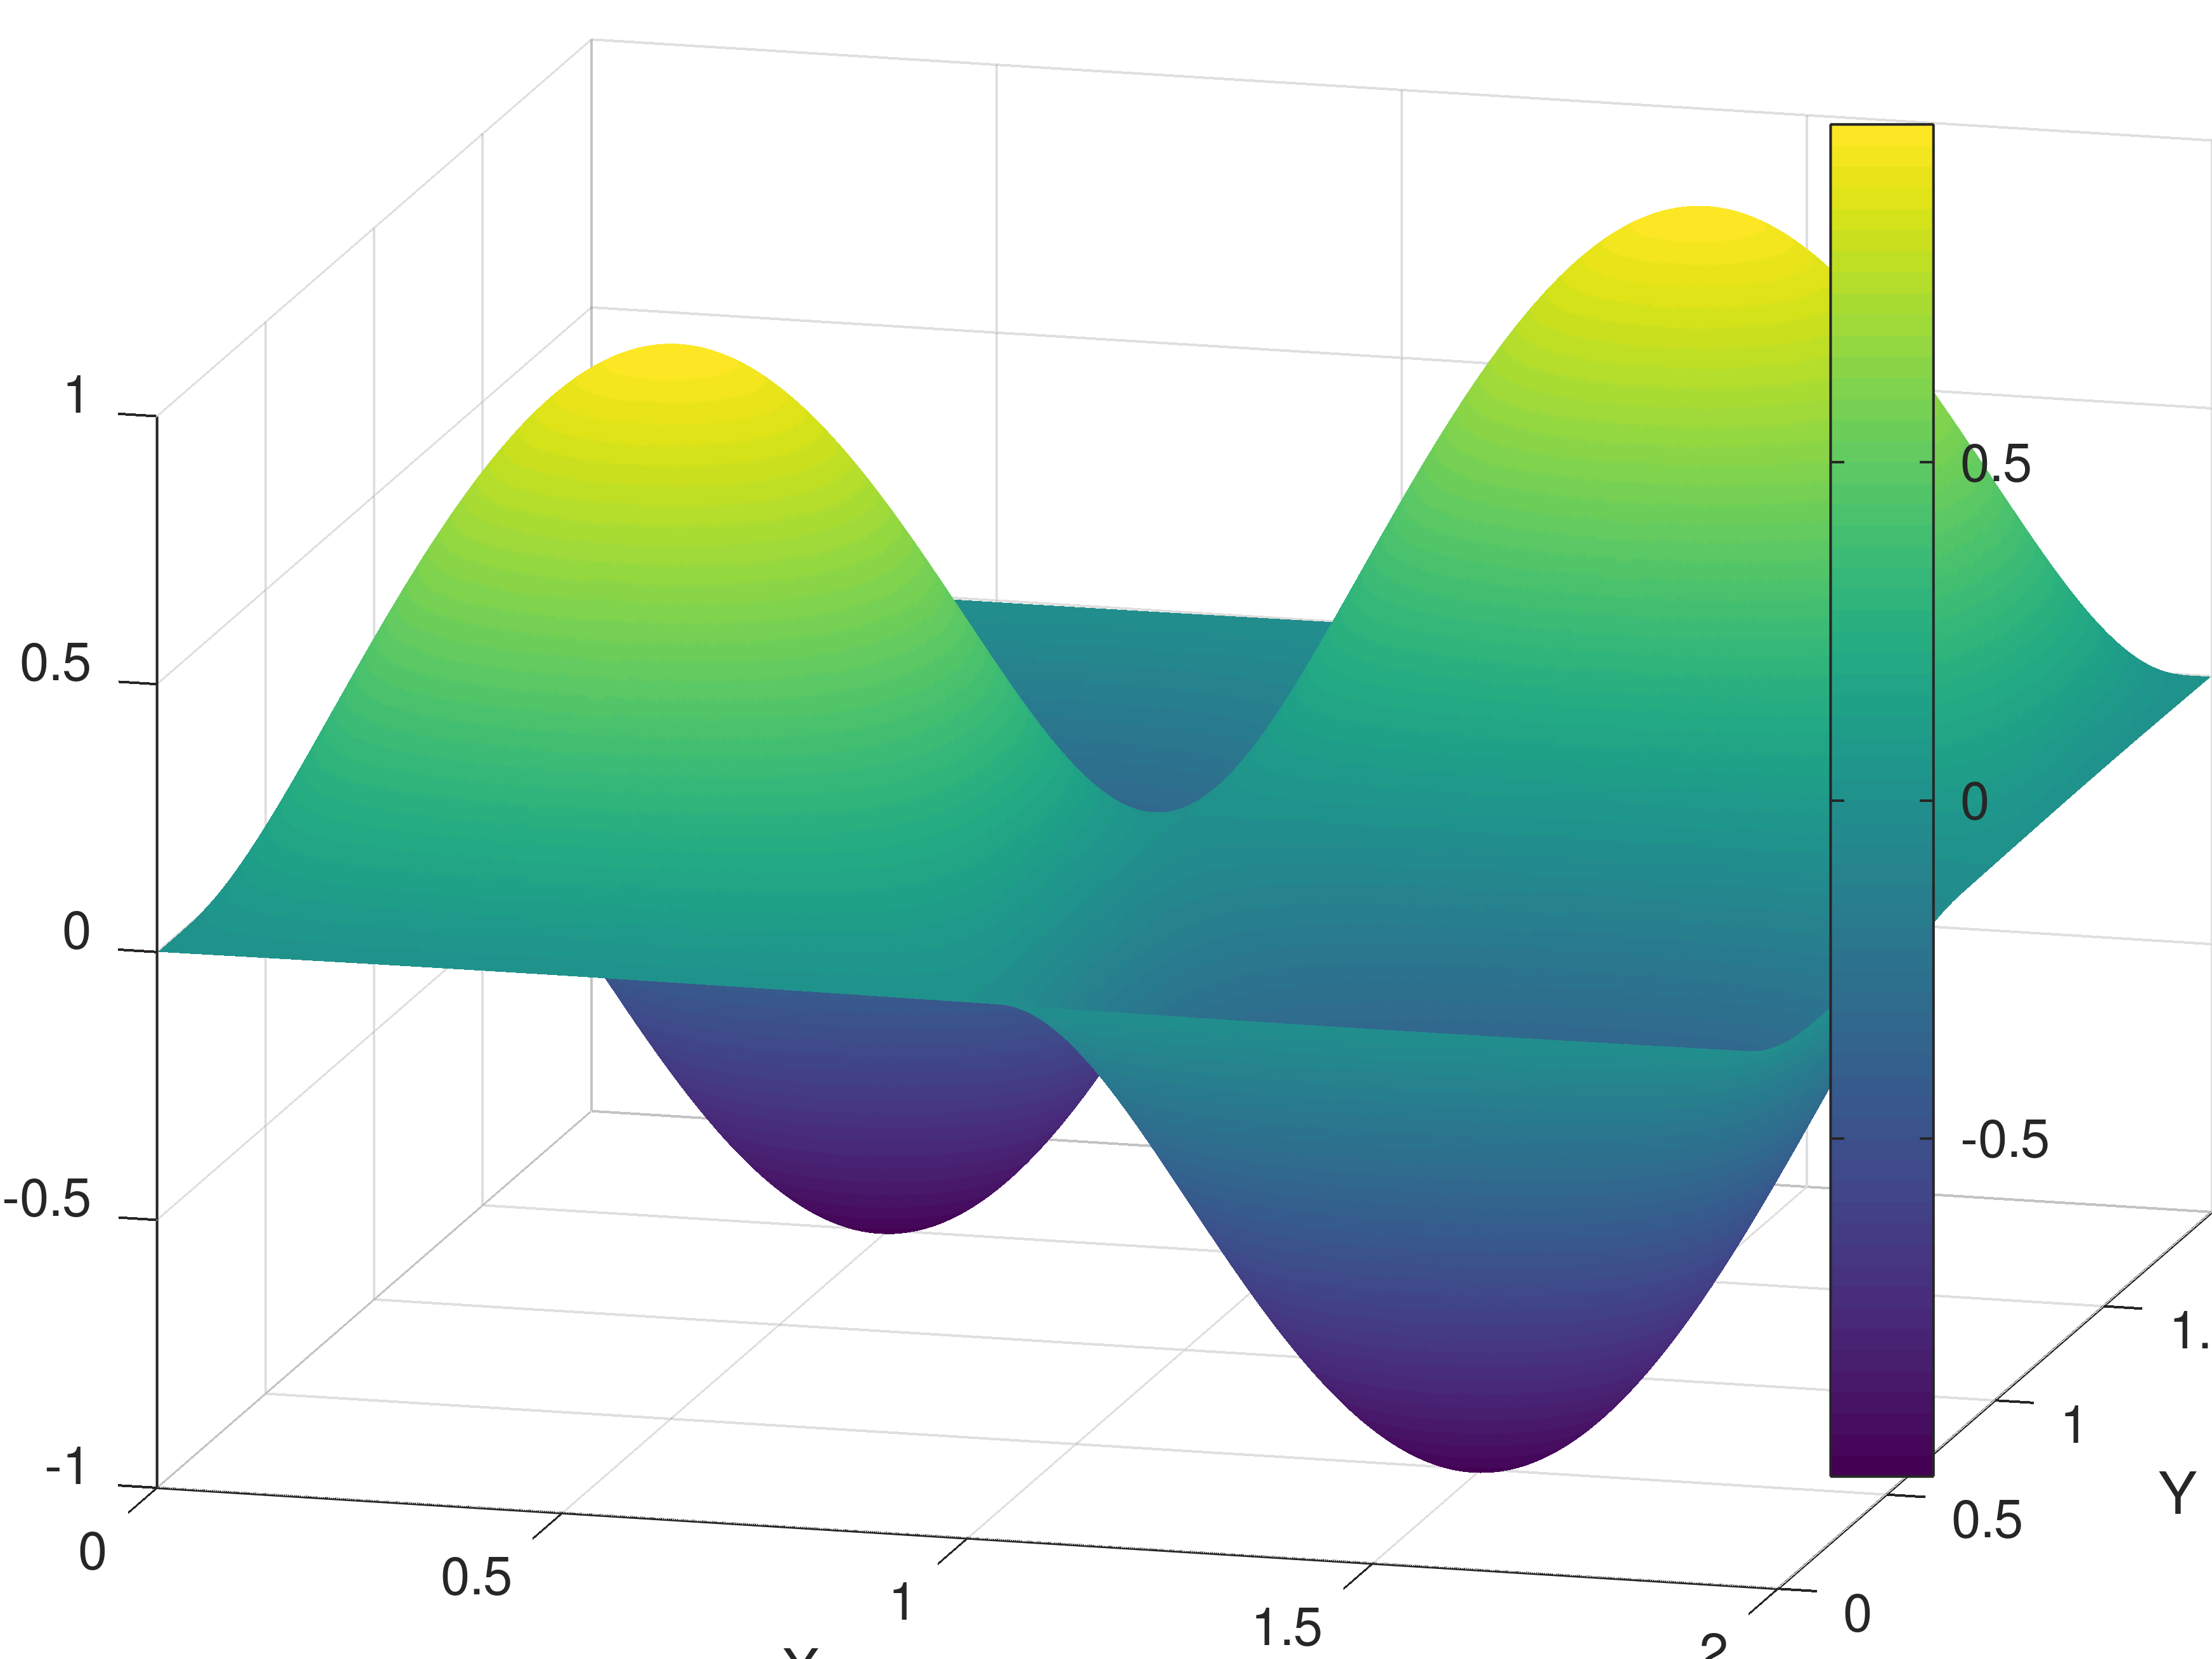
\includegraphics[width=\linewidth]{surface_hX=256_CROP_HQ1.png}
			\caption{Problema 1.}
		\end{subfigure}
		\hfill
		\begin{subfigure}{0.47\textwidth}
			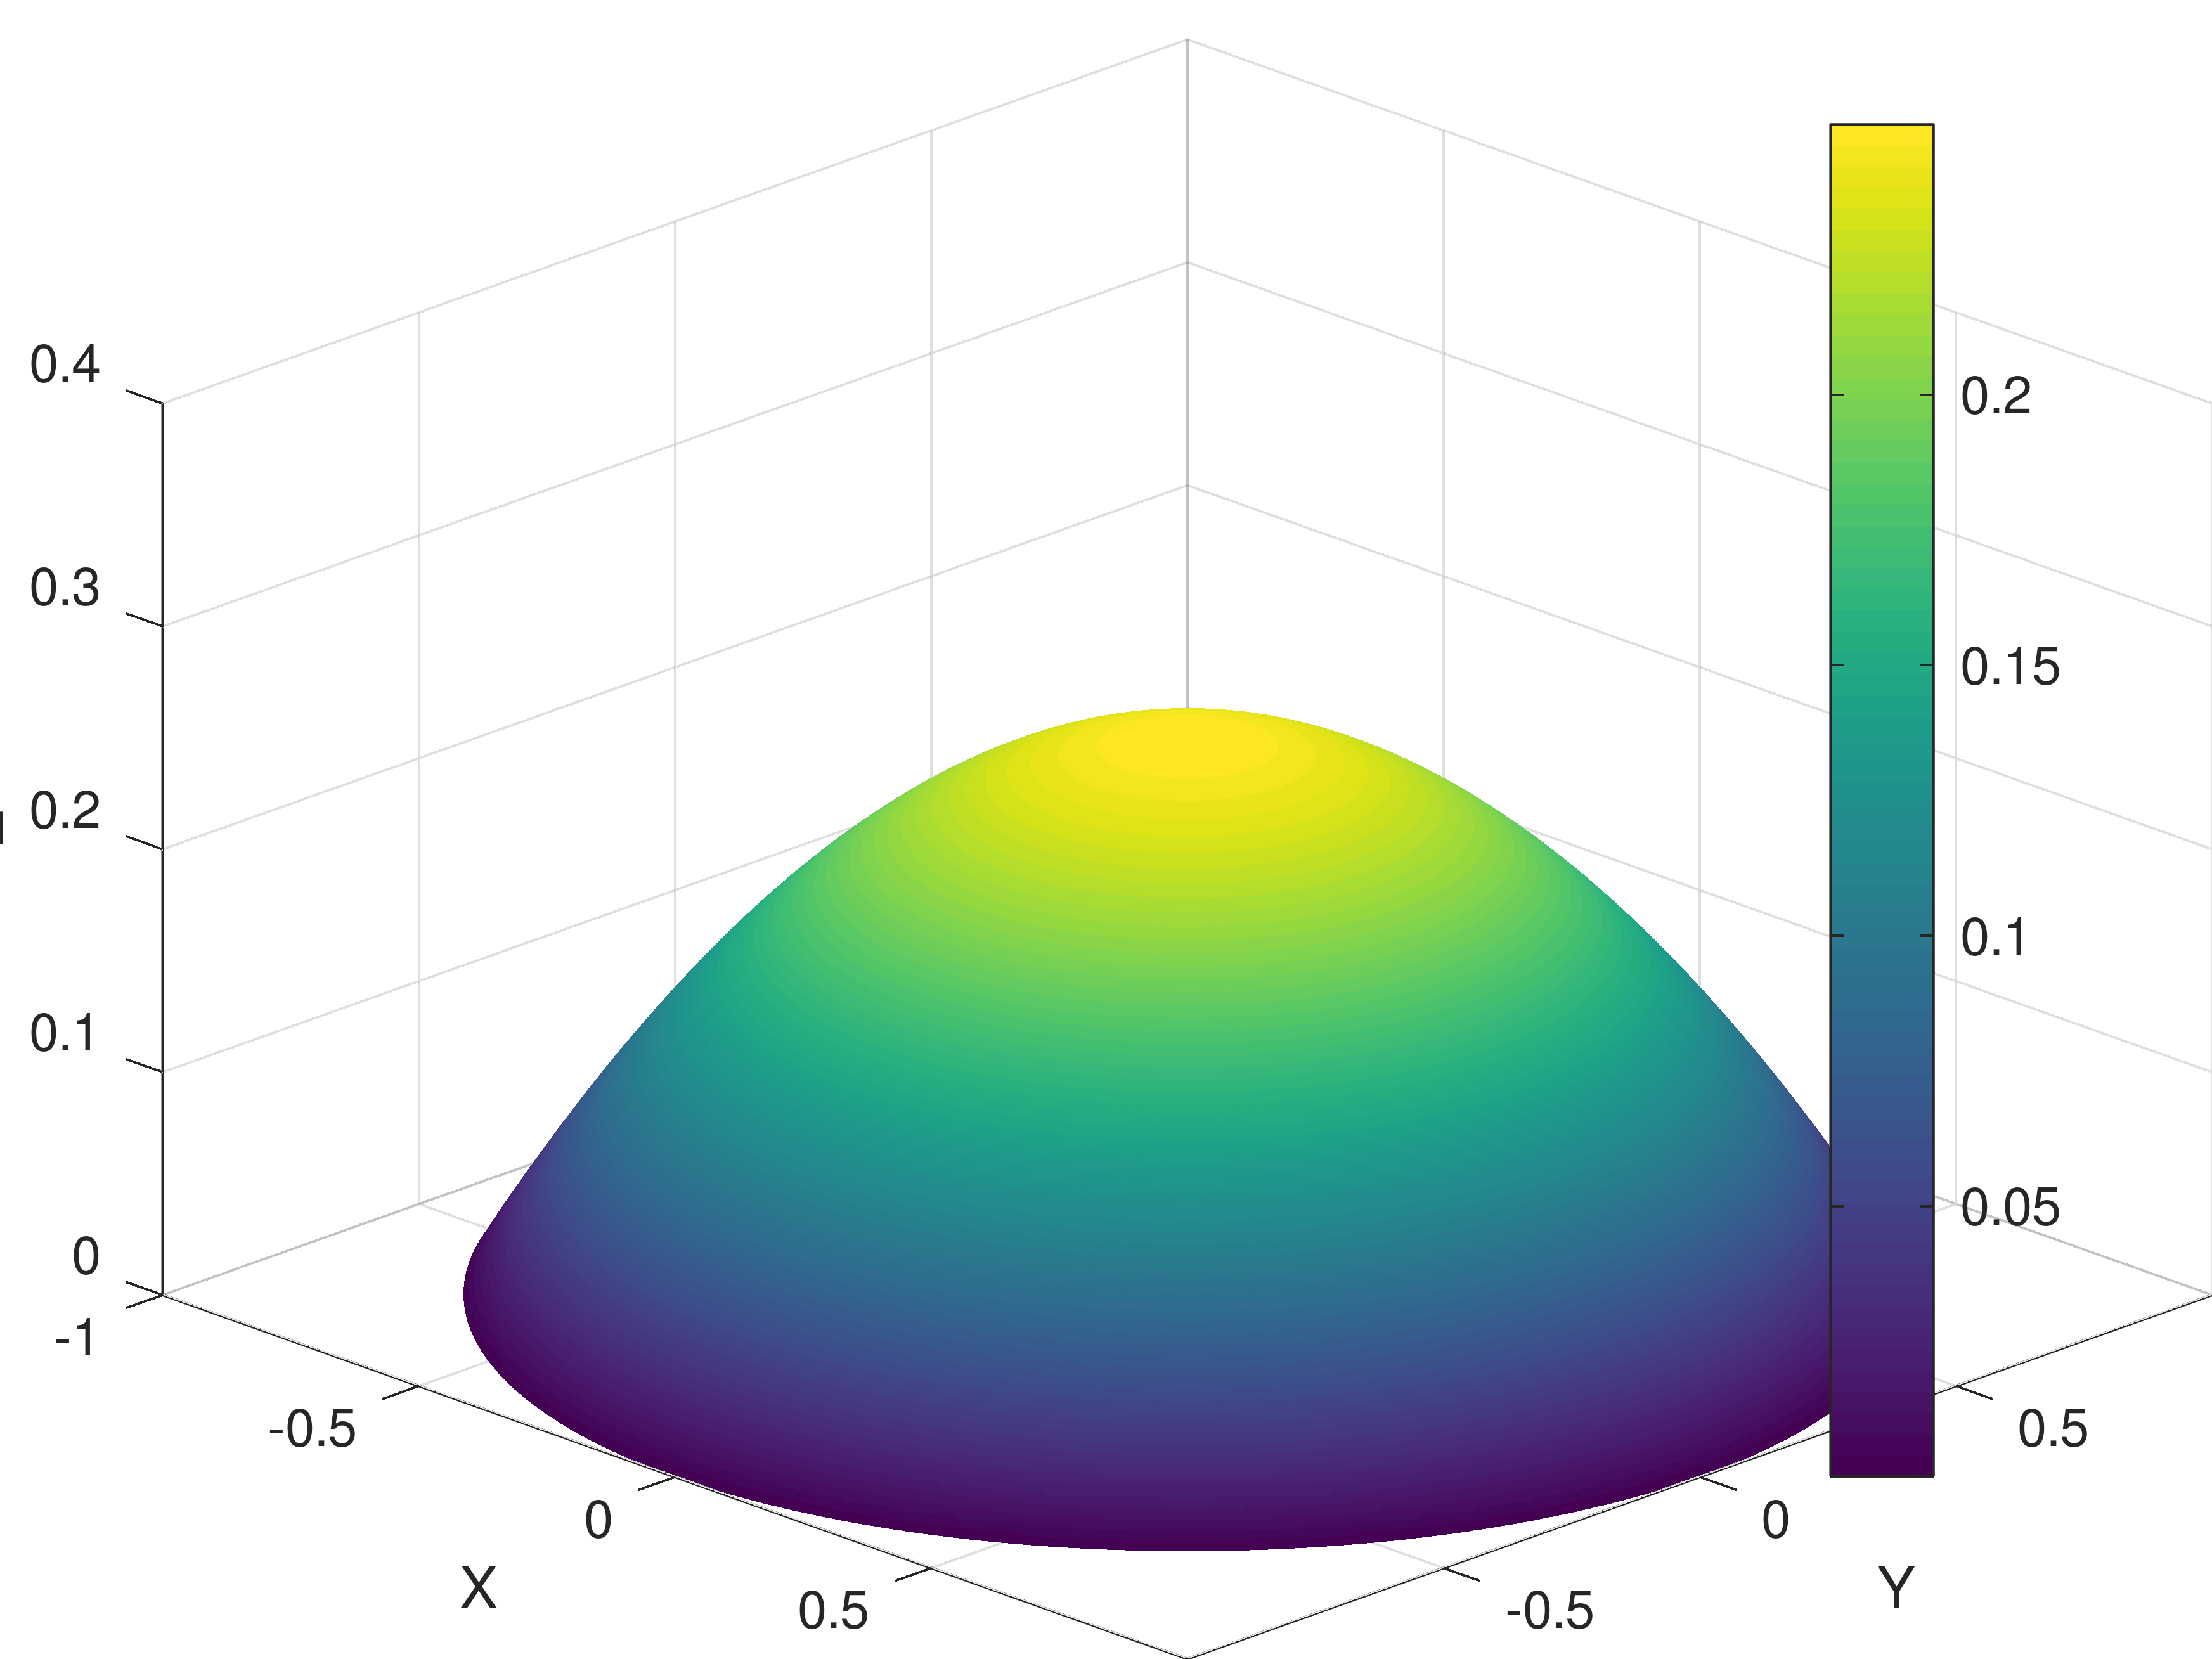
\includegraphics[width=\linewidth]{surface_hX=256_CROP_HQ.png}
			\caption{Problema 2.}
		\end{subfigure}
		%\caption{Código para las figuras en el anexo}
		% --- NOTA DEL CÓDIGO FUENTE ---
		\vspace{0.5em} % Pequeño espacio vertical para separar de las subfiguras
		\begin{flushleft}
			\footnotesize{\textit{Nota}: El eje Z, originalmente constante a 0 en ambas soluciones, se ha modificado para representar el valor de la solución en cada punto.}
		\end{flushleft}
		% -------------------------------
	\end{figure}
\end{frame}
\section{Conclusiones}
\begin{frame}
	\frametitle{Conclusiones}
	\begin{itemize}
		\item \textbf{Exactitud Geométrica}.
		\item \textbf{Alta Continuidad y Suavidad}.
		\item \textbf{Convergencia Numérica}. 
		\item \textbf{Coste Computacional}.
		\item \textbf{Implementación}. 
	\end{itemize}
\end{frame}

\begin{frame}
	\frametitle{Trabajo futuro}
	\begin{itemize}
		\item \textbf{k-refinamiento}.
		\item \textbf{Refinamiento local (T-Splines)}.
		\item \textbf{Problemas dependientes del tiempo}.
		\item \textbf{Comparación de cotas respecto a FEM}.
	\end{itemize}
\end{frame}
%------------------------------------------------

%----------------------------------------------------------------------------------------
%	CLOSING SLIDE
%----------------------------------------------------------------------------------------

\begin{frame}[plain] % The optional argument 'plain' hides the headline and footline
	\begin{center}
		{\Huge ¡Gracias por su atención!}
		
	\end{center}
\end{frame}

%----------------------------------------------------------------------------------------

\end{document} 